\section{The Hartree-Fock Approximation}
Note: Section 4 is not missing, but rather Degenerate Electron Gases spanned two lectures. 

\subsection{Motivation and Main Idea}
The Hartree-Fock, or mean-field approximation is useful when we have an intractable 4-fermion term in the Hamiltonian, for example the Coulomb interaction term.

The idea is quite simple. We approximate the full Hamiltonian $H = H_0 + H_1$ by the ``best possible'' approximation of the form:
\begin{equation}
    H_{HF} = \sum_{\v{k}, \alpha}\e_{\alpha}^{MF}(\v{k})c_{\v{k}\alpha}^\dag c_{\v{k}\alpha}.
\end{equation}
This looks like $H_0$ from before, but the modified dispersion relation allows for a tractable calculation.

\subsection{Heuristic Approach}
We first go for an intuitive approach, and then proceed with an approach that casts the problem in a variational setting (placing it on better footing). We consider:
\begin{equation}
    \begin{split}
        H_0 &= \sum_{\v{k}\alpha}\e_0(\v{k})c_{\v{k}\alpha}^\dag c_{\v{k}\alpha}
        \\ H_1 &= \frac{1}{2}\sum_{\v{kpq}\alpha\beta}V(\v{q})c^\dag_{\v{k} + \v{q}\alpha}c^\dag_{\v{p} - \v{q}\beta}c_{\v{p}\beta}c_{\v{k}\alpha}
    \end{split}
\end{equation}
Next, we ``decouple'' $H_1$ using the operator identity:
\begin{equation}
    AB = A\avg{B} + \avg{A}B - \avg{A}\avg{B} + (A - \avg{A})(B - \avg{B})
\end{equation}
This is useful as if we just focus on the last term, this is just the fluctuation of operator $A$ around its mean field value time the fluctuation of $B$ around its mean field value. The idea of mean-field theory is to say that the product of (small) fluctuations is small, and we therefore can neglect it. The central idea of the mean-field approach is to replace such products with the first three terms in the above operator identity.

Remark: in some sense, we assume that the fluctuations are small before we know what the solutions are, so we do not necessarily a priori know this will be the case. However, in practice this approach is greatly successful for the majority of problems in CM physics (the remaining 1\% of problems for which it fails tend to be interesting research problems).

Looking at our interaction term $H_1$, we have two ways to pair up our operators ($A = 13$ and $B = 24$ or $A = 14$ and $B = 23$). Let's go ahead with trying this simplification for our Hamiltonian.

\begin{equation}
    \begin{split}
        H_1^{MF} &= \frac{1}{2}\sum_{\v{kpq}\alpha\beta}V(\v{q})\left[c^\dag_{\v{k} + \v{q}\alpha}c_{\v{k}\alpha}\avg{c^\dag_{\v{p} - \v{q}\beta} c_{\v{p}\beta}} + \avg{c^\dag_{\v{k} + \v{q}\alpha}c_{\v{k}\alpha}}c^\dag_{\v{p} - \v{q}\beta} c_{\v{p}\beta} - \avg{c^\dag_{\v{k} + \v{q}\alpha}c_{\v{k}\alpha}}\avg{c^\dag_{\v{p} - \v{q}\beta} c_{\v{p}\beta}}\right.
        \\ &- \left.c^\dag_{\v{k} + \v{q}\alpha}c_{\v{p}\beta}\avg{c^{\dag}_{\v{p} - \v{q}\beta}c_{\v{k}\alpha}} - + \avg{c^\dag_{\v{k} + \v{q}\alpha}c_{\v{p}\beta}}c^{\dag}_{\v{p} - \v{q}\beta}c_{\v{k}\alpha} + \avg{c^\dag_{\v{k} + \v{q}\alpha}c_{\v{p}\beta}}\avg{c^{\dag}_{\v{p} - \v{q}\beta}c_{\v{k}\alpha}}\right]
    \end{split}
\end{equation}
Why do we include both pairings (the other pairings are dropped, but are zero in the Fermi sea)? Aren't we overcounting? In fact we are not (and careful thought shows this is not the case); this will become clearer when we do this variationally.

This looks intimidating, but there are some nice simplifications; we have two terms that come out:


for example, (s):
\begin{equation}
    \begin{split}
        \avg{c^{\dag}_{\v{p} - \v{q}\beta}c_{\v{p}\beta}} &= \delta_{\v{q} = 0}\avg{c^{\dag}_{\v{p}\beta}c_{\v{p}\beta}}
        \\ \avg{c^{\dag}_{\v{p} - \v{q}\beta}c_{\v{k}\alpha}} &= \delta_{\alpha\beta}\delta_{\v{p} - \v{q} = \v{k}}\avg{c^{\dag}_{\v{p}\beta}c_{\v{p}\beta}}
    \end{split}
\end{equation}
where the delta shows up as the product vanishes unless we are looking at the same spin with the same momentum. The first line is the direct, or \emph{Hartree} term. The second line is the exchange, or \emph{Fock} term. Taking into account these simplifications, the mean field for the Hartree-Fock Hamiltonian takes the form:
\begin{equation}
    H^{MF} = \sum_{\v{k}\alpha}\left[\e_{0}(\v{k}) + V(0)\sum_{\v{p}\beta}\avg{c^{\dag}_{\v{p}\beta}c_{\v{p}\beta}} - \sum_{\v{p}}V(\v{p} - \v{k})\avg{c^\dag_{\v{p}\alpha}c_{\v{p}\alpha}}\right]c_{\v{k}\alpha}^\dag c_{\v{k}\alpha}.
\end{equation}
So we have that:
\begin{align*}
    \e_{\alpha}^{MF}(\v{k}) = \e_{0}(\v{k}) + V(0)\sum_{\v{p}\beta}\avg{c^{\dag}_{\v{p}\beta}c_{\v{p}\beta}} - \sum_{\v{p}}V(\v{p} - \v{k})\avg{c^\dag_{\v{p}\alpha}c_{\v{p}\alpha}} = \e_{0}(\v{k}) + \e_{dir} + \e_{ex}(\v{k})
\end{align*}
where the second term is the Hartree term and the third term is the Fock term.

\subsection{Applying Hartree-Fock to Coulomb}
Let's work this out for the Coulomb interaction:
\begin{align*}
    V(\v{q}) = \frac{e^2}{V}\frac{4\pi}{q^2}
\end{align*}
Note that there is no Hartree term as $q \neq 0$. We work out the exchange term:
\begin{equation}
    \begin{split}
        -\e_{ex}(\v{k}) &= \frac{4\pi e^2}{V}\sum_{\v{p}}\frac{\theta(k_F - \v{p})}{(\v{p} - \v{k})^2} = 4\pi e^2 \int \frac{d^3p}{(2\pi)^3}\frac{\theta(k_F - \v{p})}{(\v{p} - \v{k})^2}
        \\ &= \frac{e^2}{2\pi^2}2\pi \int_0^{k_F} \int_0^\pi d\theta\sin\theta\frac{1}{p^2 + k^2 - 2pk\cos\theta}
        \\ &= \frac{e^2}{2\pi}\int_0^{k_F}p^2dp \int_{-1}^1 \frac{dz}{p^2 + k^2 - 2pkz}.
        \\ &= \frac{e^2}{k\pi}\int_0^{k_F} dp p\left[\ln\abs{\v{k} - \v{p}} - \ln\abs{\v{k} + \v{p}}\right]
        \\ &= \frac{e^2k_F}{\pi}\left[1 + \frac{k_F^2 - k^2}{2k_Fk}\ln\left|\frac{k + k_F}{k - k_F}\right|\right]
    \end{split}
\end{equation}
where we use the cosine rule in the second line, and make the substitution $\cos\theta = z$ in the third. So, we can write the final result as:
\begin{equation}
    \begin{split}
        H^{MF} &= \sum_{\v{k}\alpha}\e(\v{k})c_{\v{k}\alpha}^\dag c_{\v{k}\alpha}
        \\ \e(\v{k}) &= \e_0(\v{k}) - \frac{2e^2}{\pi}F(\frac{k}{k_F})
        \\ F(x) &= \frac{1}{2} + \frac{1-x^2}{4x}\ln\left|\frac{1 + x}{1-x}\right|
    \end{split}
\end{equation}
$F$ is plotted in Fig. \ref{fig-Fplot}.

\begin{figure}[htbp]
    \centering
    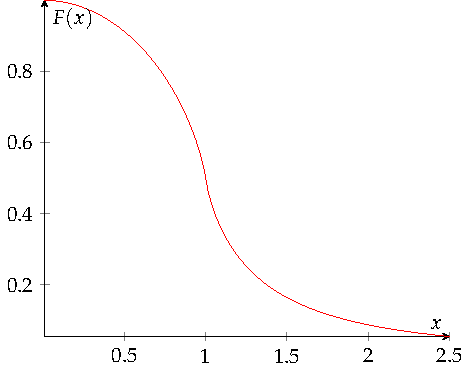
\includegraphics[]{Images/fig-Fplot.pdf}
    \caption{Plot of the function $F(x) = \frac{1}{2} + \frac{1-x^2}{4x}\ln\left|\frac{1 + x}{1-x}\right|$ which appears in the mean-field Hamiltonian dispersion relation. Note the divergence of $F'$ at $x = 1$ ($k = k_F$).}
    \label{fig-Fplot}
\end{figure}

We also recall the dispersion relation for free electrons:
\begin{align*}
    \e_0(\v{k}) = \frac{\hbar^2\v{k}^2}{2m}.
\end{align*}
We can plot the two dispersion relations side-by-side to compare them; this is done in Fig. \ref{fig-MFdispersionplot}.

\begin{figure}[htbp]
    \centering
    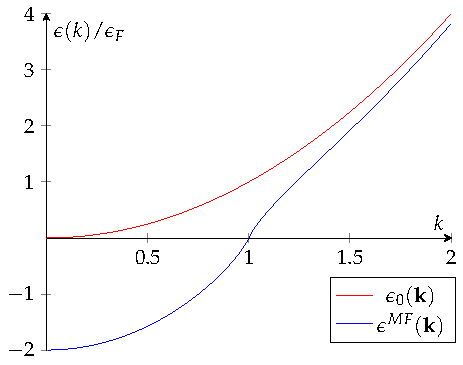
\includegraphics[]{Images/fig-MFdispersionplot.pdf}

    \caption{Plot of the free electron dispersion relation and the mean-field Hamiltonian dispersion relation. For the sake of plotting, we set $k_F =  1$.}
    \label{fig-MFdispersionplot}
\end{figure}

Note that at $k = k_F$, there is an unphysical divergence in $\nabla_\v{k}\e(\v{k})$. See HW1Q3 for more discussion of this problem, and how it can be remedied; namely, the source of the issue is the long-range Coulomb interaction. If we take into account screening, the problem goes away.

\subsection{Hartree-Fock as a Variational Bound}
Let us try to find the best possible $\e(\v{k})$ through the variational principle. We will look for $\e_0(\v{k}) + \eta_{\alpha\v{k}}$ with $\eta_{\alpha\v{k}}$ the variational parameter such that $\avg{H}_{MF}$ field is minimized. This expectation value is with respect to the ground state of the mean-field Hamiltonian.

This seems strange; we normally fix a Hamiltonian and then pick states over which we conduct an energy minimization. Here, the parameters appear in the mean-field Hamiltonian, but then the MF hamiltonian is sufficiently simple such that we know what the ground state is. So, the variational parameters directly determine the ground state of $H_{MF}$ which is the state we look at the expectation values for. Explicitly:
\begin{equation}
    \avg{H_0}_{MF} = \sum_{\v{k}\alpha}\e_0(\v{k})\avg{c^\dag_{\v{k}\alpha}c_{\v{k}\alpha}}_{MF} = \sum_{\v{k}\alpha}\e_0(\v{k})n_{\v{k}\alpha}
\end{equation}
\begin{equation}
    \begin{split}
        \avg{H_1}_{MF} &= \frac{1}{2}\sum_{\v{kpq}\alpha\beta}V(\v{q})\left[\avg{c^\dag_{\v{k} + \v{q}\alpha}c_{\v{k}\alpha}}_{MF}\avg{c^\dag_{\v{p} - \v{q}\beta}c_{\v{p}\beta}}_{MF} - \avg{c^\dag_{\v{k} + \v{q}\alpha}c_{\v{p}\beta}}_{MF}\avg{c^\dag_{\v{p} - \v{q}\beta}c_{\v{k}\alpha}}_{MF}\right]
        \\ &= \frac{1}{2}\sum_{\v{kpq}\alpha\beta}V(\v{q})\left[\delta_{\v{q} = 0}n_{\v{k}\alpha}n_{\v{p}\alpha} - \delta_{\v{k} + \v{q} = p}\delta_{\v{p} - \v{q} = \v{k}}\delta_{\alpha\beta}n_{\v{k}\alpha}n_{\v{p}\beta}\right]
        \\ &= \frac{1}{2}\left[V(0)\left(\sum_{\v{k}\alpha} n_{\v{k}\alpha}\right)^2 - \sum_{\v{k}\v{p}\alpha}V(\v{k} - \v{p})n_{\v{k}\alpha}n_{\v{p}\alpha}\right]
    \end{split}
\end{equation}
We get these pairings via the same ``destroy an electron in the Fermi sphere and then recover it'' argument we covered when discussing the second quantized form of the Jellium model. We now wish to minimize these expectation values w.r.t. our variational parameter $\eta$. One must remember that $\eta$ is implicitly hidden inside of the $n$s. We minimize via a chain rule:
\begin{equation}
        0 = \dpd{\avg{H}_{MF}}{\eta_{\v{q}\lambda}} = \sum_{\v{q}'\lambda'} \dpd{\avg{H}_{MF}}{n_{q'\lambda'}}\dpd{n_{q'\lambda'}}{{\eta_{\v{q}\lambda}}}
\end{equation}
and from this we obtain:
\begin{equation}\label{eq-lec512}
    \sum_{\v{k}\alpha}\left[e_0(\v{k}) + V(0)\sum_{\v{p}\beta}n_{\v{p}\beta} - \sum_{\v{p}}V(\v{k} - \v{p})n_{\v{p}\alpha}\right]\dpd{n_{q'\lambda'}}{{\eta_{\v{q}\lambda}}} = 0
\end{equation}
To solve this, consider:
\begin{equation}\label{eq-lec513}
    \dpd{\avg{H_{MF}}_{MF}}{\eta_{\v{q}\lambda}} = n_{\v{q}\lambda} + \sum_{\v{k}\alpha}\left[\e_0(\v{k}) + \eta_{\v{k}\alpha}\right]\dpd{n_{q'\lambda'}}{{\eta_{\v{q}\lambda}}}
\end{equation}
So substracting \eqref{eq-lec513} from \eqref{eq-lec512}, we obtain:
\begin{equation}
    \sum_{\v{k}\alpha}\left[-\eta_{\v{k}\alpha} + V(0)\sum_{\v{p}\beta}n_{\v{p}\beta} - \sum_{\v{p}}V(\v{k} - \v{p})n_{\v{p}\alpha}\right]\dpd{n_{\v{k}\alpha}}{\eta_{\v{q}\lambda}} = n_{\v{q}\lambda} -  \dpd{\avg{H_{MF}}_{MF}}{\eta_{\v{q}\lambda}}
\end{equation}
The solution is:
\begin{equation}
    \begin{split}
        \eta_{\v{k}\alpha} &= V(0)\sum_{\v{p}\beta}n_{\v{p}\beta} - \sum_{\v{p}}V(\v{k} - \v{p})n_{\v{p}\alpha}
        \\ n_{\v{q}\lambda} &= \dpd{\avg{H_{MF}}_{MF}}{\eta_{\v{q}\lambda}} = \avg{c^\dag_{\v{q}\lambda}c_{\v{q}\lambda}}_{MF}
    \end{split}
\end{equation}
It is easy to lose sight of what is being done through the many lines of writing, but one notices with the result that we have obtained the heuristic result using a very different method!

One way of justifying why the two approaches coincide; if we assume that the Hamiltonian takes the simple variational form, then the product of fluctuations that we have neglected in the heuristic approach exactly vanish; the operator approximation becomes exact.

We will not use this result immediately, but when we discuss tight-binding models and superconductivity, these approaches will be exceedingly useful.

Next time, we will discuss screening; when a test charge is put into an electron gas, there will be no long range interactions as the Coulomb force is screened by the cloud of electrons. Please by Wednesday read p.337-339 of A\&M; this is the ``Screening (General)'' section.